\documentclass[pdftex,11pt]{article}
\usepackage{amsmath}
\usepackage{caption}
\usepackage{graphicx}
\usepackage{import}
\usepackage[hmargin=1in,vmargin=1in]{geometry}
\usepackage{hyperref}
\usepackage{cleveref}
\usepackage{multicol}
\usepackage[square,sort,comma,numbers]{natbib}
\usepackage[abs]{overpic}
\usepackage{setspace}
\usepackage{subcaption}
\usepackage{wrapfig}
\usepackage[upright]{fourier} 
\usepackage[usenames,dvipsnames]{xcolor}
\usepackage{tkz-euclide}
\usepackage{listings}
\usepackage{amsmath}
\usepackage{epstopdf}

\usetkzobj{all} 
\usepackage{float}
\restylefloat{table}

\renewcommand*\thesection{\arabic{section}}

\hypersetup{
    pdfborder = {0 0 0}
}

\onehalfspacing

\begin{document}

\begin{titlepage}

\newcommand{\HRule}{\rule{\linewidth}{0.5mm}} % Defines a new command for the horizontal lines, change thickness here

\center % Center everything on the page

%----------------------------------------------------------------------------------------
%	LOGO SECTION
%----------------------------------------------------------------------------------------


\includegraphics{RU_INF_SEAL}\\[1cm] % Include a department/university logo - this will require the graphicx package
 
%----------------------------------------------------------------------------------------
 
%----------------------------------------------------------------------------------------
%	HEADING SECTIONS
%----------------------------------------------------------------------------------------

\textsc{\LARGE Rutgers, the State University of New Jersey}\\[1.5cm] % Name of your university/college
\textsc{\Large Data Structures \& Algorithms Group Paper}\\[0.5cm] % Major heading such as course name
%\textsc{\large Minor Heading}\\[0.5cm] % Minor heading such as course title

%----------------------------------------------------------------------------------------
%	TITLE SECTION
%----------------------------------------------------------------------------------------

\HRule \\[0.4cm]
{ \huge \bfseries Bitcoin: An Empirical Study of Cryptocurrency}\\[0.4cm] % Title of your document
\HRule \\[1.5cm]
 
%----------------------------------------------------------------------------------------
%	AUTHOR SECTION
%----------------------------------------------------------------------------------------


{ \Large \emph{Group 1:} \\Elie Rosen \\ Eric Wengrowski \\ Gradeigh D. Clark \\ Xianyi Gao \\}




%----------------------------------------------------------------------------------------
%	DATE SECTION
%----------------------------------------------------------------------------------------

{\large \today}\\[3cm] % Date, change the \today to a set date if you want to be precise


\vfill % Fill the rest of the page with whitespace

\end{titlepage}

\tableofcontents
\newpage

\begin{abstract}
Bitcoin exploded onto the internet scene in 2009 and became recognized as the first successful implementation of a digital currency. In this paper, we aim to discuss the history, ideas, and motivations behind digital currencies as a concept. We will motivate the issues that stopped the early adoption of a currency and explain, in some detail, how Bitcoin solves those problems. We will discuss in depth the algorithm and program flow logic involved in using Bitcoin and show complexity analysis of its algorithms as implemented in the source code. Results indicate that the hashing process is O(N) and transaction parsing operates at O(logN), while building the merkle tree O($N^2$). 
\end{abstract}

\section{Introduction}
Digital currency (or: electronic money) has been an attractive concept dating as far back as the late 20th century, when the world experienced the widespread proliferation of the internet and personal computing. The advantages were readily apparent --  a well implemented digital currency could facilitate transactions easily over the internet without any direct form of contact between parties. One would no longer need the bank to act as a third party to protect money or to mediate transaction disputes.[1] The transaction would be quick and painless -- a debit from an account on one PC to a credit on another and one that could be easily reversible. A well implemented digital currency can preserve anonymity in transactions since the two parties don't need to have any knowledge or contact, just the intent to exchange goods for a store of value. The transaction fees associated with storing money in a bank would be eliminated since the PC/internet would act as a wallet for the user and, unless the user wants to charge themselves, thus no need for a fee. Moreover, it meant there could be a greater integration of world economies through the internet; a digital currency could allow for fast money transfer across countries, oceans, and continents without the wait times or latencies associated with depositing, withdrawing, and converting between fiat currencies of overseas institutions. [1]

What happened instead was a mapping of current physical transactions onto a digital landscape. Widely adopted cryptocurrency was mostly usurped by the rise of digital banking and escrow services.  The banking industry got extended onto the internet and users turned to having to rely on third parties to verify transactions. To make purchases over the internet required a {\bf \em trusted} third party financial institution (a bank), acting as the holder of a user's money, authorizing the transfer of money to a vendor. There is no direct money transfer between two people -- only between a third party authorized to act as a monetary exchange on the internet and the vendor. This is the mapping of physical transactions on a digital landscape, only that exchanges on the internet are more limited than they are in the physical world. Transaction fees didn't disappear, waiting times didn't vanish (many transactions are sent in escrow or need to be verified e.g. Paypal), and fast money transfer still takes between one week to a month.

And then, finally, in 2009 a person operating under the pseudonym Satoshi Nakamoto published a paper outlining the requirements and algorithms necessary to implement the first successful digital currency -- Bitcoin. As it turns out, there were myriad technical challenges that needed to be overcome before a digital currency could be viably implemented. In this paper, we aim to give a strong background motivating the ideas behind the digital currency problems and how Nakamoto and Bitcoin solves those problems. Herein, we  illustrate how Bitcoin works and give practical results regarding the algorithms it uses to solve digital currency problems. 

\section{Problem}
The biggest problem that faced digital currency is called the {\bf double-spending} problem.[1][2][10] Double-spending refers to the act of using one piece of currency to perform two transactions. What is important to note here is that this is not the same as splitting the currency into multiple parts.[2] An example of double-spending is using one dollar bill in two different vending machines to get multiple items for the same dollar. This became an issue in digital currency because records and files that stored transaction history were susceptible to corruption or duplication. With a virtual transactions, there's never a true guarantee that someone has transferred their file of currency without keeping a copy for themselves;[1] it would require the system to be entirely free of corruption. Double-spending is the main reason why financial transactions online are done through trusted third parties -- there is someone verifying that a transaction has occurred and money has changed hands. Of course, we note that a successful digital currency shouldn't need to rely on a third party.[1]

Effectively, this double-spending problem boils down to an issue of trust between two parties. One party can't ensure that the other party isn't acting in an untrustworthy manner, i.e. spending their money in multiple places. The only way currencies, economies, and monetary systems work is if there is trust in the system.[2] Without trust, there is no way to exchange a store of value for goods -- it's back to direct exchange. So the algorithmic problem that arises here is actually an old problem known in computer network known as {\bf Byzantine Generals}.[10] 

Byzantine Generals is a problem that uses a framing device of two generals attempting to attack an army to illustrate the issues that arise when trying to communicate information over a network connection that is unreliable. The story goes as follows. Two generals are attempting to coordinate an attack against an enemy army. General A needs to send a message to General B to tell them that they need to attack at dawn. A messenger for General A is dispatched and sent to General B. However, there is no guarantee that General B received the message from General A's messenger. General B can try to abate this by dispatching another messenger to General A to say that he agrees with the arranged attack time. But there's no guarantee his message reaches General A. And the problem goes on like this {\em ad nauseum}.[10]

Digital currencies fall short the above problem exactly. The bitcoin solution to this problem is to announce all transactions publicly, eliminating the need for an omniscient, trusted third party.[8] Parties attempting to communicate with each other perform {\bf proof-of-work}. The work proof requires nodes in the network to store complete {\bf global history} locally.[1][2] 

Proof-of-work schemes are not new concepts. A simple example of proof-of-work would be CAPTCHA image schemes. When a user wants to sign up for an online service, they will encounter some CAPTCHA bar asking them to enter the characters in an image. By entering the characters, a person is doing work to prove that they are human and not a robot. On the computer side, proof of work is done by asking a computer to do some calculation and send it back. 

To keep the generals synchronized on everything is going on requires a global history.[8] No party should act without referring to the history to see what the other party {\em has done} and sees confirmation of what the other party {\em will do}. This global history is meant to be expanded to every actor in the global market, forming a history for every user that can be checked to determine how much money every person has by checking their transaction history and adding it all up. So now currency is no longer files that are transferred between people (like dollar bills), but additions and subtractions on a public ledger.[8] Transactions are added to the ledger when people agree that have transactions have taken place. So together, the proof-of-work and the global history solve the Byzantine Generals problem.

However, the public history gives rise to another issue: false histories.[1][2] The double spending problem arose from the inability to trust the actions of the actors in the economic system. But now that there is a history, what stops the untrustworthy actors from creating false histories and collaborating on it by verifying false transactions?  If there are collaborating liars that can perform the proof-of-work in unison to lie then the system doesn't work. So this is two problems, actually: one problem is making transactions using other people's money and the other problem is that there isn't a unified agreement on a true history.[1]

Satoshi's Bitcoin employs simple solutions to these issues. First, to ensure that one party doesn't make transactions for another party, the system should implement public-private key cryptography. A user can sign a transaction with his private key and it can be verified with his public key to show that the user is agreeing with the money being taken or received.[9] As far as the false history problem, follow the longest chain of verified history and have everyone jump to work off of that history when new history comes in.[1] In this way, it is very difficult to manufacture a false history. Since there are public and private keys, if some attacker wants to present a false history, they need to work off a transaction that was first signed off between two parties. The attacker would then start doing work from {\em that point} in the history chain and have to catch up to the current history.[1][2] This is a very expensive, very wasteful process[2] -- assuming there are honest people working off the most recent history then it would be very hard to catch up enough to overtake and invalidate it. It would require a computing power >50\% of the total power of the network.[1]

There is one final issue that is a product of Satoshi's solution -- how can the system incentivize others to verify transactions? The verification process is inherently wasteful; a computer must perform some long, otherwise wasteful calculation as a proof-of-work to add a transaction to the global history. People who verify transactions must give up electricity to do the proof-of-work, and that electricity costs money in the physical world.[2] So, as a means of incentivizing transaction verification, anyone who successfully verifies transactions are rewarded with a set number of bitcoins -- the units of the digital currency -- as a reward for contributing to the history.[1] Rewarding these people with bitcoins also allows the system to introduce new coins into circulation.[1][2]

In summary, digital currencies suffered from a double-spending problem that is similar to the structure of the Byzantine General networking problem.[1] To solve that issue, people agree on a global history of transactions between all users in the system.[8] To add transactions to the history, users in the system need to a proof-of-work problem to verify that a transaction is legitimate before it can be added to the global history.[1][2] A public-private key cryptography system is implemented to prevent users from making transactions with the money of other users and to associate transactions with a person.[1][2][9] False histories are dissuaded by having the network follow the longest verified history in the network.[1][2] People are incentivized to work on verifying transactions by being rewarded with bitcoins for their work.[1]

\section{Bitcoin Terminology}
The ideas outlined in the {\bf Problems} section are a high level abstraction of the concepts outlined by Satoshi in his paper. In this section, we will explain how the solutions are implemented. Specifically, we will look at the components that make up the global history and the proof-of-work scheme and describe them in detail.

\subsection{Transaction}

% Transaction
\begin{figure}[H]
	\centering
	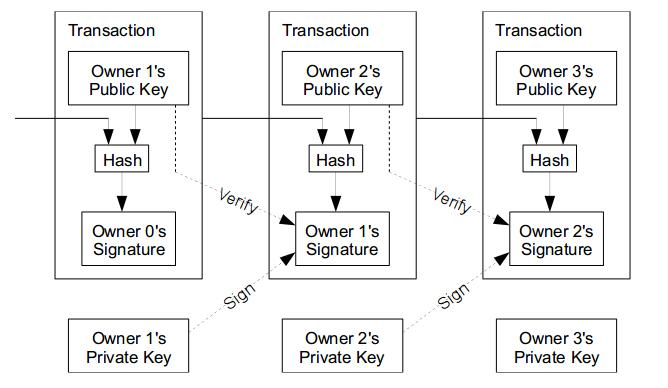
\includegraphics[width=100mm]{figures/transaction.jpg}
	\caption{Block diagram of a typical Bitcoin transaction process}
	\label{transaction}
\end{figure}

Pictured above is the general representation of a transaction inside the Bitcoin network. Transactions are the first building block of our global history network and they are composed of a series of "ins" and "outs" -- an "in" is the money going to an owner and an "out" is the money leaving an owner. A given transaction will generally contain a random number of "ins" and "outs"; there is no fixed amount -- it depends on the amount of money present in a user's wallet and the amount they are trying to send.  The components listed in the diagram are:
\begin{itemize}
	\item Owner A's public key. Owner 1 is the person receiving/sending something in a transaction.
	\item Owner 0's Signature. Owner 0 was the previous holder of some amount of currency that was signed over to Owner 1. The transaction contains this amount so that it can be verified where it came from.
	\item Hash. This is a hash of the previous transaction. This is done to assist in implementing a history between transactions; the hash of the transaction is used to easily check if an entire transaction occurred and used to effect later in constructing a Merkle tree.
	\item Owner A's private key. Owner 1 uses to tell the world that they approve of the transaction.
\end{itemize}

\subsection{Block}
A block is an entry in the global history system. It is pictured below.

% block
\begin{figure}[H]
	\centering
	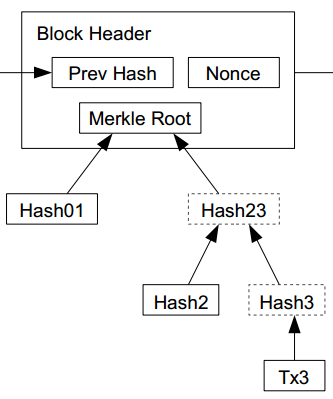
\includegraphics[width=50mm]{figures/block.png}
	\caption{Breakdown of transactions included into the block header}
	\label{block}
\end{figure}

An individual block what the miners perform the proof of work problem to solve. Miners are repeatedly hashing the block information in an attempt to obtain a hash value that can be considered a potential match to a block. The picture above represents Satoshi's view of the block and not what is ultimately implemented by Bitcoin. It is more educational to examine the hardware structure of the block instead since that is what needs to be hashed.

In hardware, the block is represented as an 80 byte array composed of the following components:

\begin{table}[H]
	\centering
 	\begin{tabular}{|p{2.25cm}|p{5cm}|p{5cm}|p{1cm}|}
		\hline
		\textbf{Field} & \textbf{Purpose} & \textbf{Updated when\dots}  & \textbf{Size (Bytes)}\\
		\hline
 		Version & Block version number & You upgrade the software and it specifies a new version & 4\\  \hline  
		hashPrevBlock & 256-bit hash of the previous block header &  A new block comes in & 32  \\  \hline 
		hashMerkleRoot & 256-bit hash based on all of the transactions in the block & A transaction is accepted & 32 \\  \hline 
		Time   & Current timestamp as seconds since 1970-01-01T00:00 UTC & Every few seconds & 4 \\  \hline 
		Bits & Current target in compact format & The difficulty is adjusted & 4  \\  \hline 
		Nonce &32-bit number (starts at 0) &A hash is tried (increments) & 4  \\  \hline 
	\end{tabular}
	\caption{Components to the blockheader data structure}	
\label{tab:blockheader}
\end{table}

From this table, we can ascertain that a block contains the following elements:
\begin{itemize}
	\item Nonce. This is a 32 bit number that is routinely incremented when searching for a hash solution. Its only purpose is to be changed on each hash iteration.
	\item Merkle root. This is the root of the Merkle Tree, a binary tree constructed of hashes of the transactions that are being verified with that block. This Merkle root is how the transactions are linked into the block.
	\item Previous hash. This is the hash of the previous block. If we are working off a global history, then the current history should have an idea of what happened before so that the current block can be traced back to where it came from.
	\item Time. This is used to determine at what point the block was verified. Note: The timestamp on verified blocks are often unreliable because clever miners will vary the timestamp once they exhaust all nonce values.
	\item Bits. This is a misleading name meant to refer to the current target as a 4 byte number. The target is what miners compare to when they are searching for a block solution; if the hash attempt is less than the target then a successful block has been found.
	\item Version. This is the current software version that Bitcoin is running at.
\end{itemize}

\subsection{Blockchain}
The blockchain is the distributed global history that was alluded to in the Problems section. It is pictured below

%blockchain
\begin{figure}[H]
	\centering
	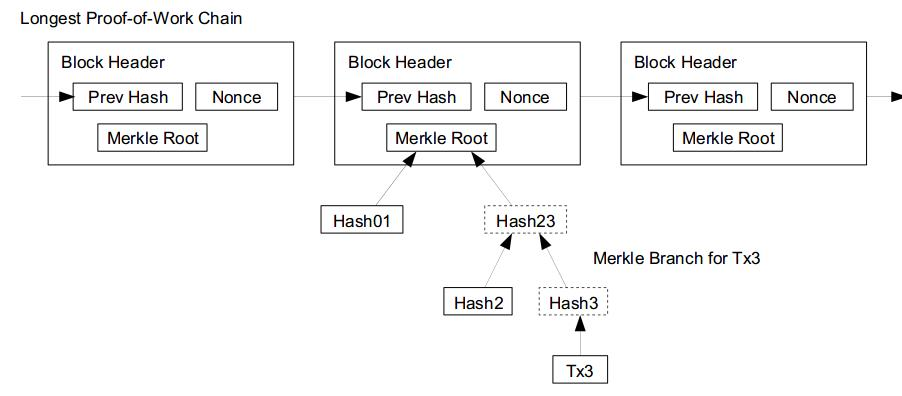
\includegraphics[width=100mm]{figures/blockchain.jpg}
	\caption{Full chain of blocks that show the proof-of-work chain}
	\label{blockchain}
\end{figure}

The blockchain is a connection of {\bf blocks} together that form the proof-of-work history chain. Blocks are chained together via their hash values; the way to find the previous block in the chain is to check the hash of the block header until a match is found.

\section{Data Structures \& Algorithms Employed }
The Bitcoin process is fully decentralized, where all of the work to maintain the integrity of the network is based off of the peer-to-peer structure of the mining network. The structure of the Bitcoin blockchain requires that all miners keep a copy of the working Merkle tree ( the longest chain of agreed blocks). The file size is large (~15 GB) but necessary to verify transactions. The SHA256 hashing algorithm is used to find possible solutions to be awarded Bitcoins.

\subsection{Merkle Tree}
A Merkle tree is a binary tree where every non-leaf node is a hash of its immediate children. Refer to the figure below:
% Merkle Tree
\begin{figure}[H]
	\centering
	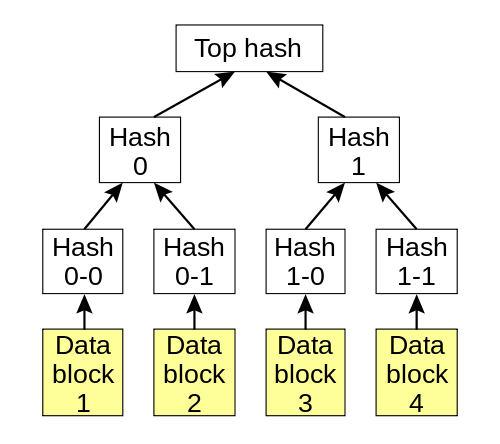
\includegraphics[width=100mm]{figures/merkletree.png}
	\caption{Merkle Tree block diagram}
	\label{merkletree}
\end{figure}

So unlike a regular binary tree, the insertion process doesn't start with the root. Instead, all of the (planned) insertions begin as leaves of the tree. For our process, the Data blocks represent transactions and NOT blocks in the blockchain. In the pre-insertion stage, all inserted values are paired up in sets of 2; if there is an odd number of leaves then that leaf is paired up with itself. Insertion begins immediately from the leaf down; each transaction is hashed and inserted directly into the tree at the bottom. Then, a recursive process occurs to implement the tree. The paired leaves are concatenated with one another to form a double length value and is then hashed to form the parent of the concatenated children. This process continues until, finally, there are only two hashes left to concatenate and subsequently hash. At that point, the final hash and inserted value into the tree is the root of the Merkle tree.
So, the operations for constructing the tree are:
\begin{itemize}
	\item Gather up the transactions you want to verify
	\item Hash them
	\item Insert as leaves
	\item Concatenate
	\item Hash and insert recursively until the root is obtained
\end{itemize}

\subsection{SHA256}
The SHA256 hashing algorithm was initially developed by the National Security Agency in 2001. It is a one-way hashing algorithm based off of the first 32 bits of the fractional parts of the square roots of the first 8 primes (floating point values) combined with the first 32 bits of the fractional parts of the cube roots of the first 64 primes. These values are algorithmically interesting due to their lack of relation to other values. By design, SHA256 guarantees that the output will always be 256 bits long. The hash is generated by taking the initial values and combining it with the data to be hashed through bitwise operations such as AND, XOR, and NOT. If the data to be hashed is larger than 512 bits, the data will be split into chunks where each chunk goes through the hashing process and is then added to the initial values thus creating new initial values for the next chunk. Due to this process, the time to hash a file is proportional to the size of the file. 

To relate this all to Bitcoin, we utilize the SHA256 algorithm to build carefully designed hashes that are smaller than the current target. It is impossible to guess a combination that would achieve a guess smaller than the target, instead we attempt to try as many guesses as possible to increase our chances at winning the current target. Our experiment will explore the speed it takes to hash the block header and the opportunity of winning a block potentially worth up to \$10,000.

It is important to note that all hashing done in the Bitcoin process refers to a double application of the SHA256 algorithm; every hash of SHA256 is hashed again with SHA256.

\subsection{Introduction to Mining}
The structure that enables Bitcoin mining is important to the design of the system. The mining process is supported by a system of data structures and algorithms that must be enormously scalable to support huge transaction volume. Mining is the main algorithmic point of interest in Bitcoin and is central to the operation of the network.

First of all, mining is not really the act of trying to get Bitcoins; that is secondary. Mining is rather the essential process that must be performed for monetary exchange to take place. The only way transactions can be verified in this network is for someone to do work -- that work is mining. If there is no one mining for Bitcoins then transactions will never be verified; the system will have ceased to function.
The process list is as follows:
\begin{enumerate}
	\item First, a miner will select a number of transactions that they want to verify.
	\item With the transactions, the miner will compute a Merkle tree and a Merkle root.
	\item Then, the miner will build the 80B block header that was described in {\bf Bitcoin Terminology}, starting with a nonce of 0.
	\item The miner will begin double hashing the block header.
	\begin{enumerate}
		\item If the hash is less than the current target, a block is created and added to the blockchain. The miner is rewarded with a set number of bitcoins.
		\item If unsuccessful, the miner will increment the nonce and return to step 4.
		\begin{enumerate}
			\item If the nonce is fully exhausted, the miner will change something else (the timestamp or the number of transactions) and start hashing over $2^{32}$ nonce values again.
		\end{enumerate}
		\item If a new block is found before the miner succeeds, the miner needs to update their history and start over since the block needs to have the hash of the most recent block in it.
	\end{enumerate}
\end{enumerate}

The mining process is illustrated in the flowchart below.

% Mining Steps
\begin{figure}[H]
	\centering
	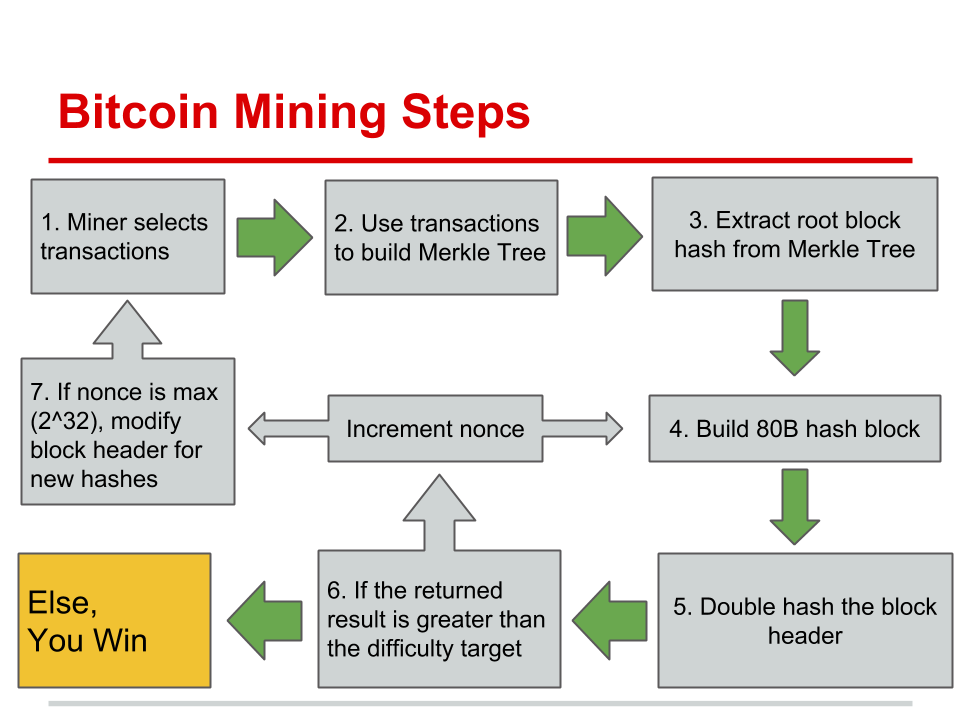
\includegraphics[width=150mm]{figures/steps.png}
	\caption{Flowchart for mining Bitcoins}
	\label{steps}
\end{figure}

\subsubsection{Pseudocode}
\begin{lstlisting}
while( /*No Change in Prev Hash Block*/ )
{
	// Compute Merkle Root
	Gather a Block of Unverified Potential Transaction from Pool
	Build Merkle Tree from Selected Transactions
	Return Block Header from Merkle Tree = hashMerkleRoot
	
	for  (Nonce = 0; Nonce < 4294967296; Nonce ++)
	{
		block = concat(Version, hashPrevBlock, hashMerkleRoot, Time, Bits, Nonce);
		hash = SHA256(SHA256(block));
		
		if (hash < Bits)
			// Winning block, Broadcast to all other nodes
	}
	// Modify Block Header
	time = CurrentTime();
}
\end{lstlisting}


\section{Experiments}
In order to examine the algorithmic performance of Bitcoin hashing, we first set up the Bitcoin block header structure to incorporate into the hash. As a reminder: the header is comprised of a version number, a hash of the previous block header, the Merkle root, the current time, the current target, and a nonce that is updated at every iteration of the hash. To this end, we considered a few iterations on Bitcoin complexity analysis:
\begin{enumerate}
	\item The Merkle tree build time is a one time expenditure. But it can still be computationally exhaustive if the number of transactions is quite large. How does the time to build the Merkle tree and extract its root hash vary with the number of transactions and can its effect on solution time be significant?
	\item The target/difficulty is the bottleneck to solving a block. How does the time to find a block vary with increasing difficulty?
	\item The difficulty affects the solution time, but the transactions affect the build time. What is the compound effect of these two processes superimposed on each other? When does one overtake the other?
\end{enumerate}

First, to implement any of this in a way that is experimentally viable requires some relaxation in the block header structure. The current difficulty of the system is far too large for us to measure real-world complexity. Bitcoin adjusts the target such that a block is solved every 10 minutes. There are miners out there working at rates much faster than a normal PC can handle so getting a solution isn't feasible. Instead, we opted to set up a Bitcoin example simulation. This assumes the following simplifications:
\begin{itemize}
	\item The version number is always "1".
	\item The current time is always updated to be the same as the program runtime.
	\item The difficulty is a variable amount that the user sets.
	\begin{itemize}	
		\item Since the operations need to be performed on byte arrays instead of integers, we used the number of leading zeros as the difficulty compare points for our experiments. This is a much simple solution than comparing to the target. So a solution is found when there are N leading zeros.
	\end{itemize}
	\item The number of transactions is a variable amount that the user sets.
	\begin{itemize}
		\item The number of inputs and outputs to a single transaction is random. As such, the transaction hashes are constructed by creating a random integer array of length equivalent to the number of transaction. The random value is equal to the average number of inputs and outputs. This is important since the storage varies with the number of inputs and outputs.
	\end{itemize}
	\item The previous hash is just a SHA256 double hash of a random number between 1 and 1000. Since we don't have prior history, we just create a random hash to work with.
\end{itemize}

Implementing the first experiment meant implementing the Merkle tree structure. It is important to keep in mind that we are most interested in the hash of the root and not so much the values that came before it. Additionally, no mining is performed on modern computers -- they are performed on ASICs and FPGAs whose language is C, so no object oriented concepts are available to use. On hardware, it is fastest to implement the Merkle tree as an ArrayList (vector). The transactions are varied and the time is recorded.

The second experiment requires varying the loop condition for the number of leading zeroes on a hash attempt. This is repeated, random hash attempts until a solution occurs. Because solutions occur randomly, we opted to perform a 20 trial average to get an idea of how long it takes on average for a solution to be found for a given difficulty. 
The third experiment requires that the difficulty be fixed at a specific value and the total runtime be measured as the number of transactions changes. Once we are done iterating over the transactions, the difficulty changes and the process repeats. Since the Merkle runtime and the hashing run time depend on different variables, it will take a 3D plot to figure out how they affect each other. 

\section{Results and Analysis}
\subsection{SHA256}
Before moving into the results of note, we will take time here to examine the runtime effect of hashing to see if it has any impact on program complexity. The results are below.

As shown in the graph, the time it takes to execute N hashes increases linearly as N gets large. This is due to the fact that  we only continually hash a modified 80 byte structure. The time it takes to hash an object is constant, and is being attempted N times. If the size of the header were to vary, we could expect that this curve would not be linear.

% SHA256
\begin{figure}[H]
	\centering
	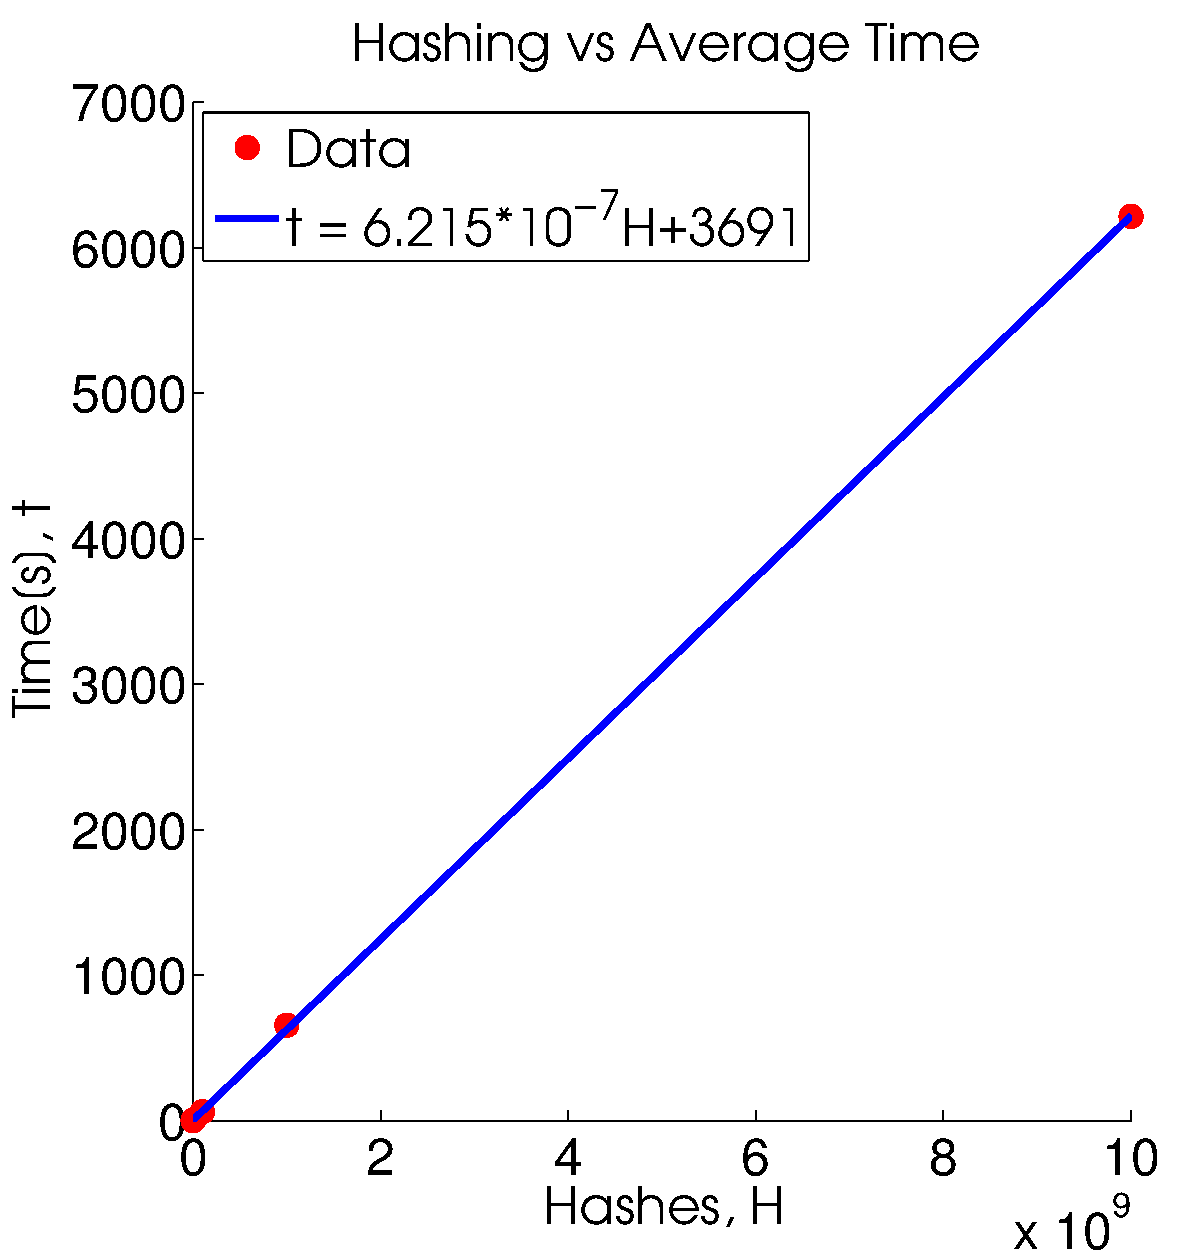
\includegraphics[width=100mm]{figures/SHA256.pdf}
	\caption{SHA256 hashing time for N trials}
	\label{sha256}
\end{figure}

As the block difficulty changes, the number of hashes needed to solve the block varies. The higher the difficulty value, the larger the number of hashes. Since guesses are generated randomly, the number of hashes to solve blocks with same difficulty also varies. In our experimental testing, we ran each case 20 times and took the average number of hashes for the results. Besides difficulty level, the number of transactions in the block also affects the number of hashes needed to solve the block. Since the hashing time is proportional to the number of hashes, more hashes result in longer time to solve the block. From the data points alone, the number of hashes required to solve a plot appeared to be either exponential or quadratic. As such, we did two least squares fits to see which one was a better fit. As it turns out, the exponential fit performed better. 

As for why, we had to consider what the computer is being asked to do. It is the attempt to impose order on a random process, i.e. require a non-random leading component (the string of zeroes) come in a fixed order. The best case analysis is that the hashing obtains the right number of leading zeroes immediately leading to O(n) = 1. The worst case analysis is a little different. It requires that, over a natural set of numbers, we can quantify the probability of obtaining a solution is, on average:

\begin{figure}[H]
	\centering
 	$P = \frac{1}{2^{32}}$
 \end{figure}

Assuming equal probability chance of obtaining an answer. The result follows naturally from assuming a Poisson random process. This assumption is valid given the fact that the path to solution is effectively like that of a lottery, where no matter how many attempts one makes that never changes the probability of success.

Note that this follows
The difficulty modulates the answer somewhat, so:
\begin{figure}[H]
	\centering
 	$P = \frac{1}{2^{32}*D}$
 \end{figure}

D denotes the difficulty.
We hash in linear time, so on average we should take:
\begin{figure}[H]
	\centering
 	$E = \frac{ht}{2^{32}*D}$.
 \end{figure}

where h is the hashrate and t is the time spent hashing. E is now the average reward rather than the average probability.


As D increases, the probability of finding a solution decreases as a scalar multiple of an exponential quantity. While we hash linearly, the attempts at finding a solution increase exponentially because that multiple reduced the chance of finding a solution by an exponential factor. This is the worst case scenario. On average, it will be something weaker but tends towards this same behavior. This is why the curve appears exponential in both the hashrate AND the time; they are modulated the same way, probabilistically speaking. 

\begin{figure}[H]
	\centering
	\begin{subfigure}[H]{0.4\textwidth}
		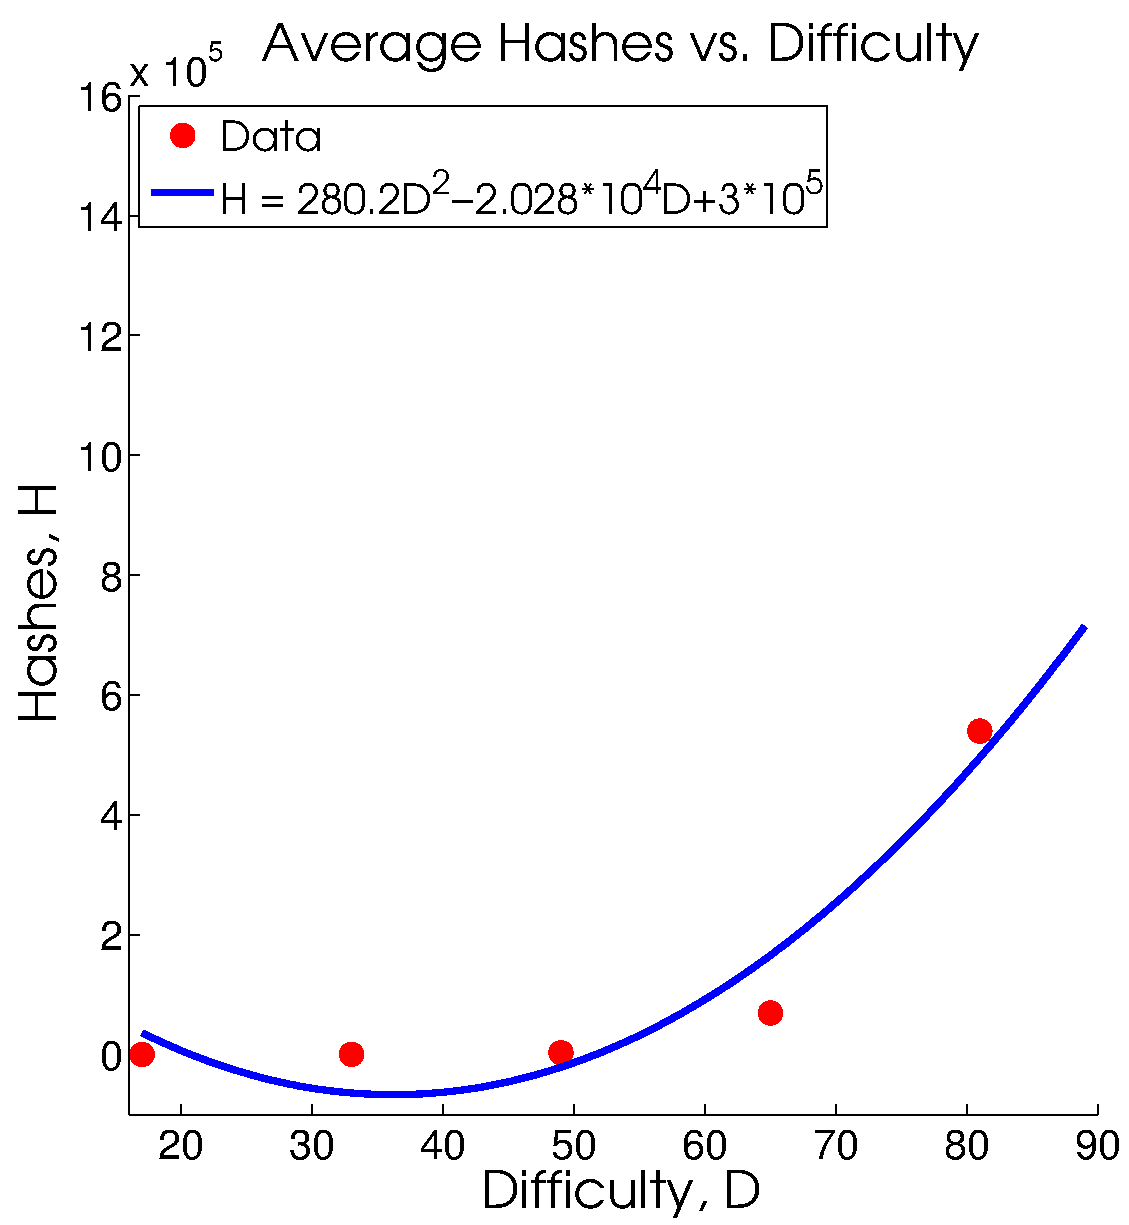
\includegraphics[width=\textwidth]{figures/Poly.pdf}
		\caption{Poly fit}
	\end{subfigure}
	\begin{subfigure}[H]{0.4\textwidth}
		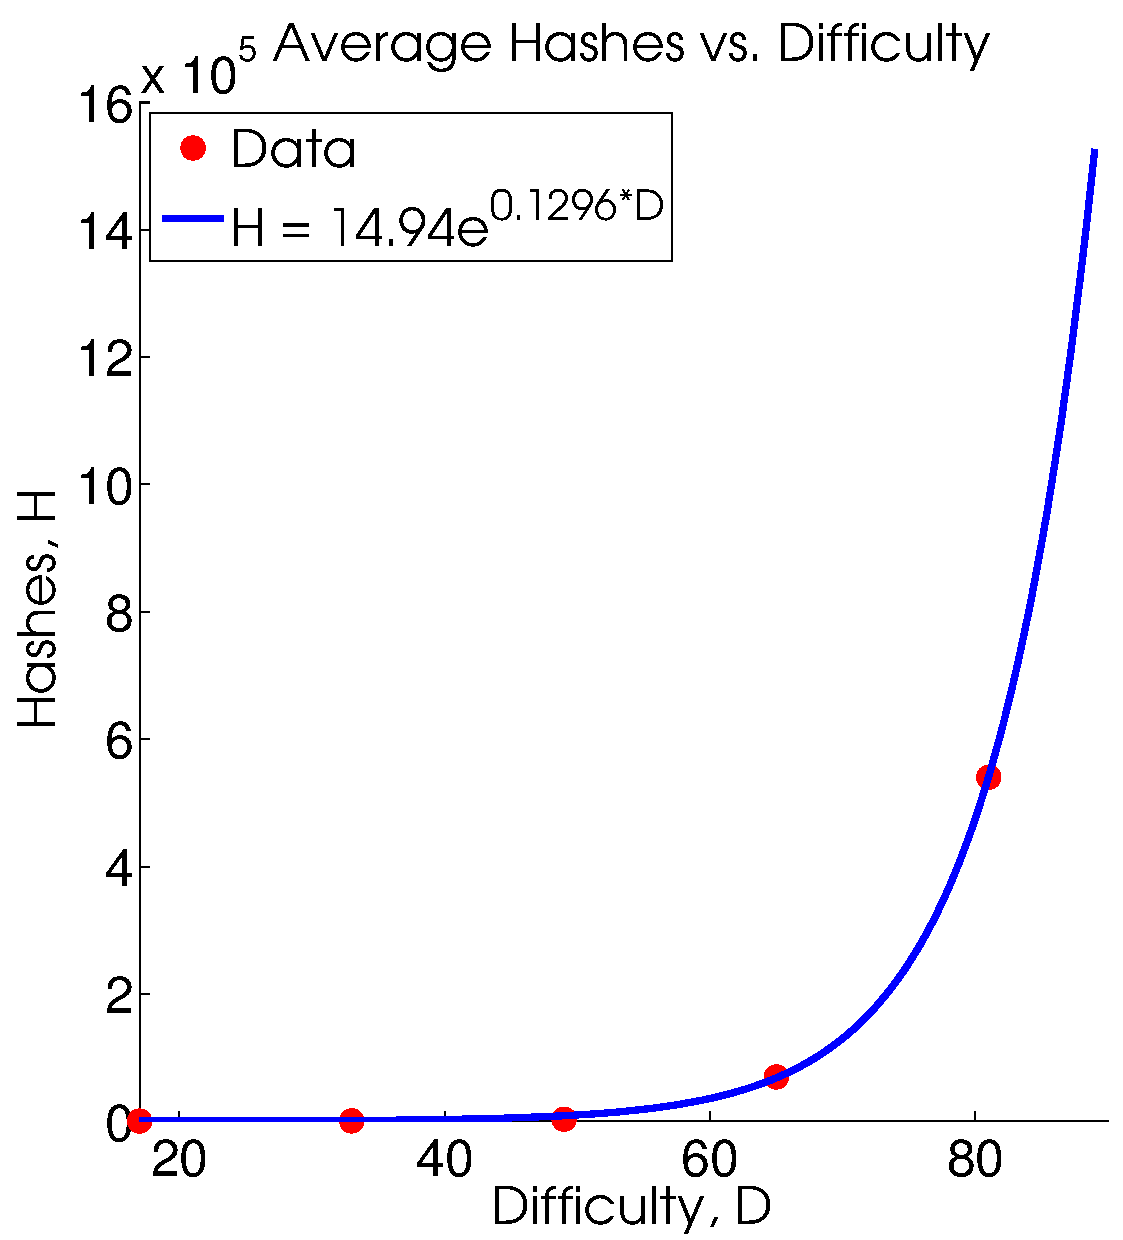
\includegraphics[width=\textwidth]{figures/Exp.pdf}
		\caption{Exponential fit}
	\end{subfigure}
	\caption{Average number of hashes required to win a block as the difficulty increases}
	\label{fig:hash}
\end{figure}

\subsection{Merkle Tree}
The number of transactions selected in Merkle Tree construction has a significant impact on construction time. We constructed Merkle Trees using the number of transactions typically hashed by actual bitcoin miners, between 100 and 1000. In the world of Bitcoin mining, time is money. So miners have an incentive to minimize the amount of computational time they spend doing anything other than generating potential blockchain guesses. Since the number of transactions hashed has no impact on the probability of a successful guess, transaction fees are the only incentive that a miner has to generate a Merkle Tree with more than 0 transactions. 

Empirical results show that growth rate of Merkle Tree build time is quadratic, with a small constant C so that  $~C*N^2$ where $C = 1.315*10^-5$. We can confirm this result theoretically as well. In the Merkle construction phase, 

Our results show that relatively little time is spent constructing the Merkle Tree, as compared to actually computing a hash that below target. Even for unusually large Merkle Trees (N = 1000) hashed at an artificially low difficulty (D = 81),  the time spent computing a successful hash is ~15 times higher. We can expect this ratio to rise further because the growth rate of Merkle tree build time is {\bf O($N^2$)}, while growth rate of difficulty to successful hash rate is {\bf O($e^D$)} or {\bf O($2^N$)}. We can conclude that although growth rate is quadratic, the cost of Merkle tree build time plays a relatively minor role in the overall time cost of mining.

\begin{figure}[H]
	\centering
	\begin{subfigure}[H]{0.4\textwidth}
		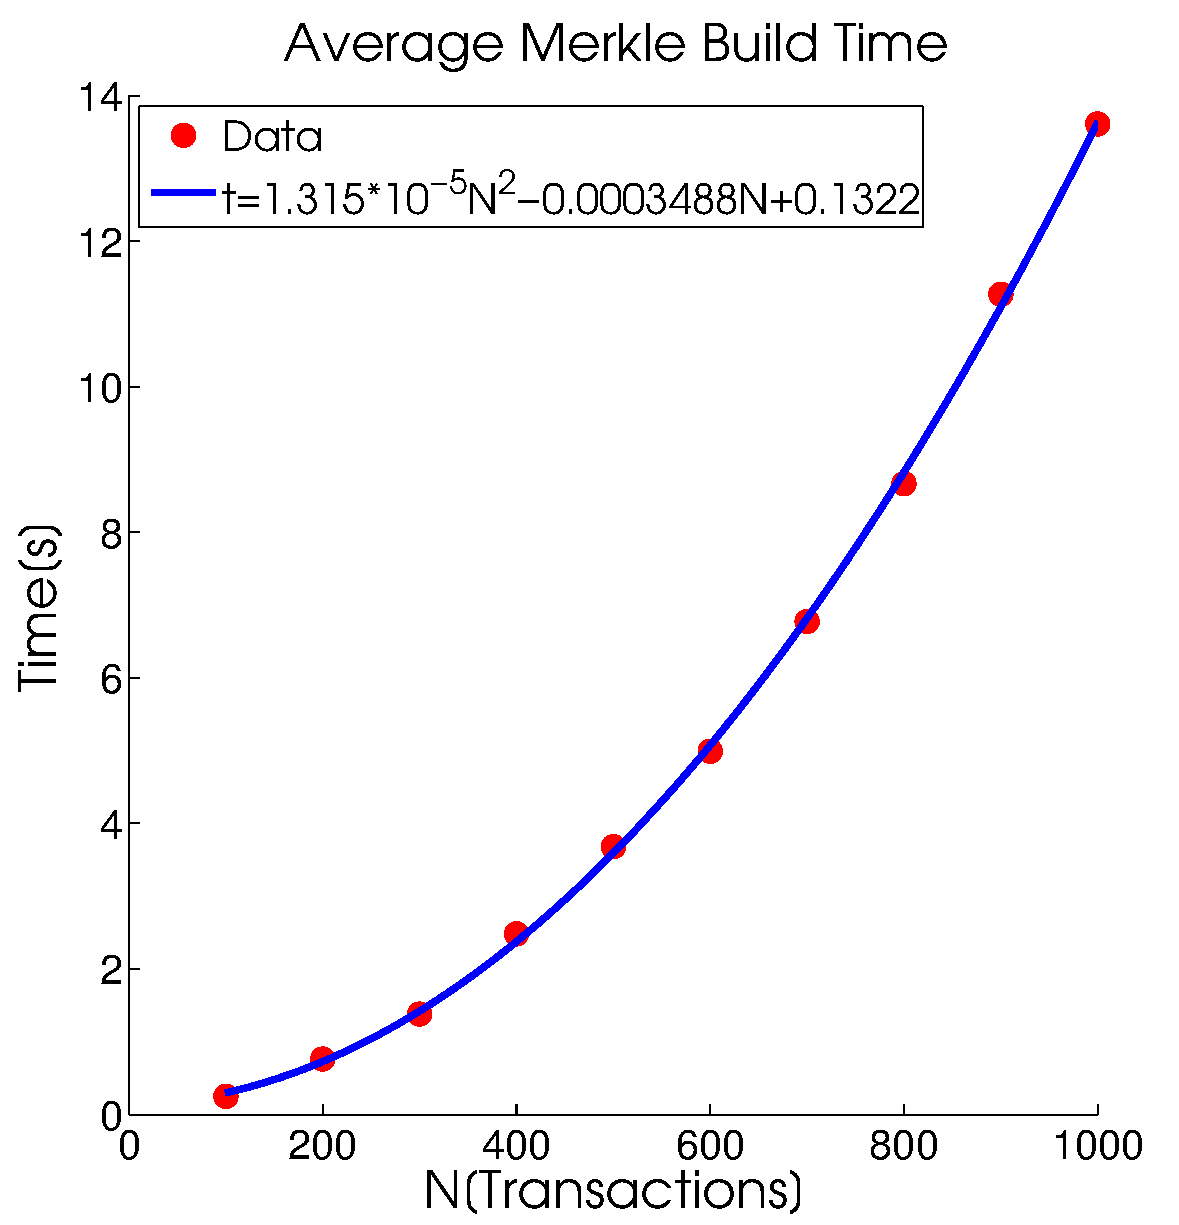
\includegraphics[width=\textwidth]{figures/MerkPoly.pdf}
		\caption{Poly fit}
	\end{subfigure}
	\begin{subfigure}[H]{0.4\textwidth}
		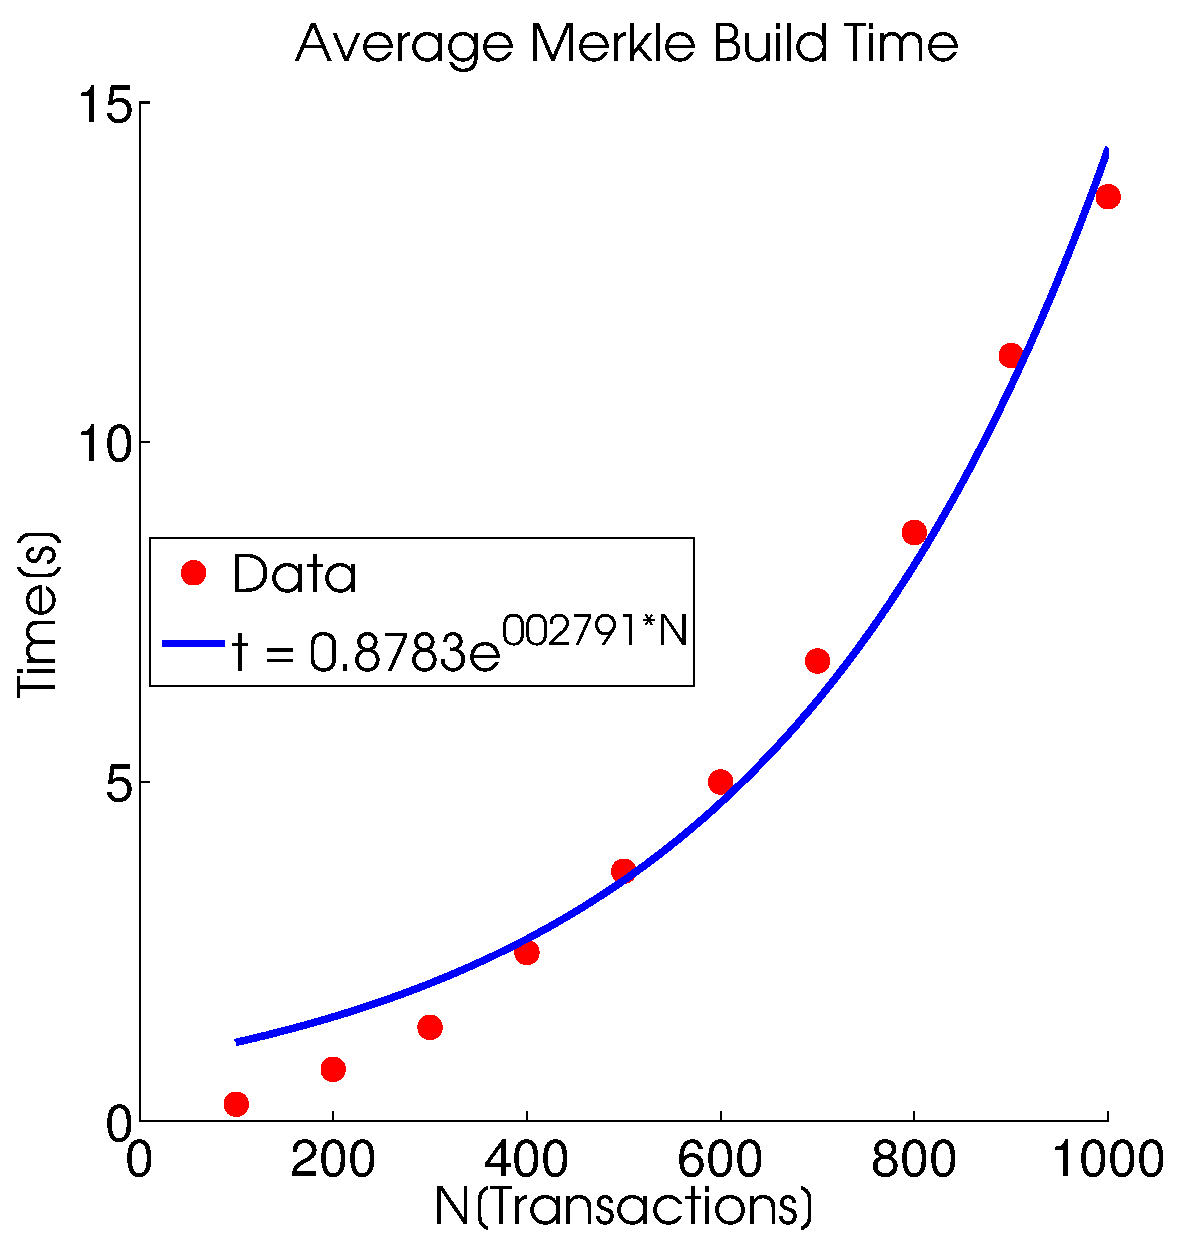
\includegraphics[width=\textwidth]{figures/MerkExp.pdf}
		\caption{Exponential fit}
	\end{subfigure}
	\caption{Average merkle tree build time as transaction count increases}
	\label{fig:merk}
\end{figure}

\subsection{Effects of Running in Real-Time}

The 3D plot below is obtained from fixing the difficulty and varying the number of transactions and then fixing the number of transactions and varying the difficulty.  To the effect of measuring whether the Merkle build time has a significant effect on the time to solution for a hash level the consensus is: not really. While the number of transactions have an effect on low difficulty levels when the number of transactions inccluded are high (1000), that effect is mitigated by the time the difficulty reaches higher peaks and really takes off. The exponential growth in time dwarfs the one-time contribution of the quadratic transaction build. 

% SolveTimeExp
\begin{figure}[H]
	\centering
	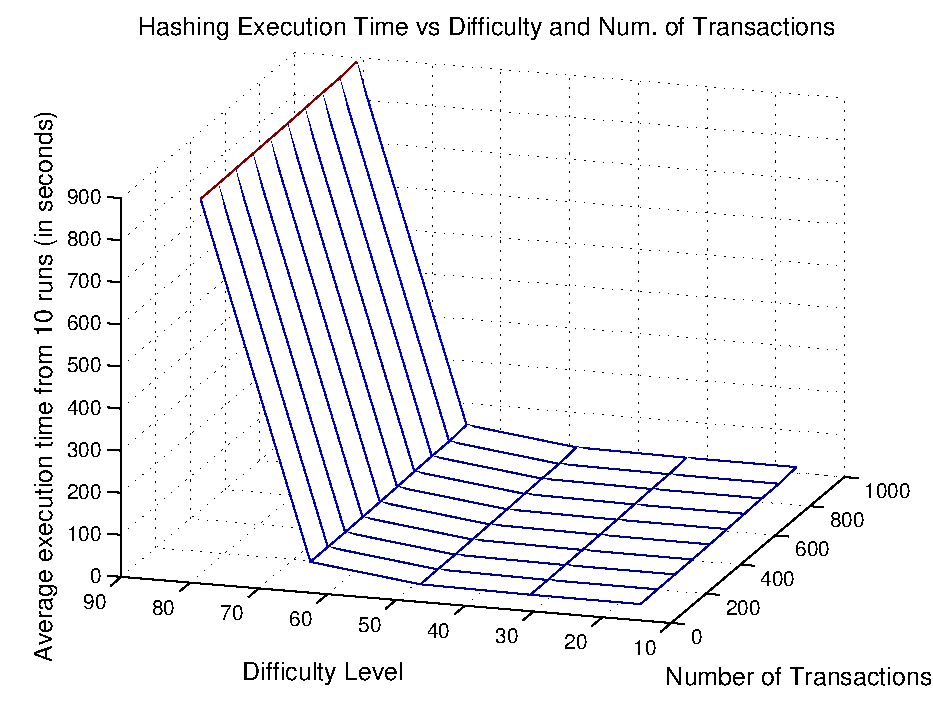
\includegraphics[width=100mm]{figures/3Dplot-eps-converted-to.pdf}
	\caption{As can be seen, the overhead from adding transactions to the merkle root becomes marginal as the difficulty increases}
	\label{3dgraph}
\end{figure}



\section{Discussion}

\subsection{Transaction Issues}
In theory, it would make sense for miners to aggregate as many transactions as possible and try to verify them as quickly as possible. But in practice, miners don't do that. The problem is that Bitcoin is a lottery system. Whoever can get the solution to the block first wins and all other takers must abandon their claim to the prize and start working on another block. As such, there is a lot of competition between miners rather than collusion. Miners are at odds with each other to obtain the block solution first. Although the process is entirely random, there is something to be said of the effect of time and hashrate. Recalling the expected value of return:

\begin{figure}[H]
	\centering
 	$E[x] = \frac{ht}{2^{32}*D}$
 \end{figure}

The time and hashrate increase the expectation of reward. Any time given up means reducing the chance of reward. So it is in the miners best interest to both hash more quickly and to increase the time spent hashing. However, if the miners are collecting a large number of transaction then the time spent before hashing is reduced. If miner A decides to aggregate 1000 transactions (~14 seconds on a CPU) and miner B decides to just take 1 transaction(~0 seconds), then miner A lost 14 seconds in the attempt for a solution. With typical machines hashing at well over 1GH/s, that means the miner missed 14*$10^{9}$ attempts at finding an answer as compared to miner B. This is a huge issue! In fact, most miners have realized this and typically shoot for somewhere between 200~400 transactions to accept in a given block rather than taking all thats available in memory. As such, our results lend an understanding to some of the unspoken nature of miner dynamics in Bitcoin.

Another effect aggregating a large number of transactions has a miner is that it increases the probability of {\bf orphaned blocks}. An orphan block occurs when two different miners obtain a block solution at approximately the same time with similar transactions being verified inside each. What happens is that this creates a fork in the blockchain; users will end up working off of one of the two sets of blocks without knowing which one is better. At some point, one of the block histories will catch ahead of the other, resulting in the other block being abandoned. This abandoned block is referred to as an orphan block. When an orphan block occurs, the reward money from those blocks is lost and any transactions inside them not verified by the longest history are sent back to the memory pool. Part of the reason orphaned blocks can occur is network latency due to building the Merkle tree. Miners hate to lose block opportunities, but they hate even more to lose money they thought they won. Many of the orphaned blocks in the blockchain have a higher number of transactions than the usual 200~400, lending credence to the idea that Merkle tree construction attributed to slowing down the miner. There's cause to believe this; a lot of transactions would increase network latency when being sent back to the blockchain, delaying the time it takes to accept a block.

\subsection{Effect of Difficulty on Hashing}
In the mining process, 80B blocks are passed through the SHA-256 hashing algorithm. The hash value that is returned is then compared against a difficulty metric. The returned value must be less than or equal to a 256-bit target. The current target is known by all users in the bitcoin network. It's value is calculated so that, on average, 1 block is hashed every 10 minutes. At this rate, 2016 blocks should be successfully hashed in a 2 week period. Once 2016 blocks are hashed, the 256-bit target value is (potentially) adjusted so that based on the rate of the previous 2016 blocks hashed, the 2 week target would have been met. The target is never modified by more than a factor of 4.[7]

Difficulty represents a ratio of entropic likelihood of a successful block hash at the current target as compared with the largest legal target value. The largest target is the value by which successful hashing is easiest, since your hash needs to be {/em less than or equal} to that value.[6] The formula for difficulty is as follows,
\begin{figure}[H]
	\centering
 	$Difficulty = \frac{largest\_legal\_target}{current\_target}$.
 \end{figure}


Essentially, difficulty is a simple numerical ratio of the easiest possible target over the current target.

The maximum target used by SHA256 mining devices in hex representation is:

\begin{figure}[H]
	\centering
 	$0x00000000FFFFFFFFFFFFFFFFFFFFFFFFFFFFFFFFFFFFFFFFFFFFFFFFFFFFFFFF$
 \end{figure}

However, since Bitcoin stores the target as a float, the value is truncated:
\begin{figure}[H]
	\centering
 	$0x00000000FFFF0000000000000000000000000000000000000000000000000000$
 \end{figure}

This leads to 2 methods of calculating difficulty: pool difficulty based on full precision ({\em pdiff}), and the difficulty as estimated by Bitcoin clients ({\em bdiff}).

For example, the current target (4/11/2014, 21:48) is: 
\begin{figure}[H]
	\centering
 	$0x0000000000000000B3AA00000000000000000000000000000000000000000000$
 \end{figure}


Therefore, the current {\em pdiff} is:
\begin{figure}[H]
	\centering
 	$\frac{0x00000000FFFFFFFFFFFFFFFFFFFFFFFFFFFFFFFFFFFFFFFFFFFFFFFFFFFFFFFF}{0x0000000000000000B3AA00000000000000000000000000000000000000000000} = 6119819470.16$
 \end{figure}

And the current {\em bdiff} is:
\begin{figure}[H]
	\centering
 	$\frac{0x00000000FFFF0000000000000000000000000000000000000000000000000000}{0x0000000000000000B3AA00000000000000000000000000000000000000000000} =  6119726089.1281$
 \end{figure}

From the above information, we can conclude that the collective pool of Bitcoin miners are 6119819470.16 times less likely to successfully hash 1 block attempt than the case with the largest target. 

This difficulty metric gives us a method of directly comparing successful hashing probability. This allows members of the bitcoin network to accurately adjust the difficulty so that the next set of 2016 blocks will be hashed in precisely 2 weeks. However, this estimation is based on the assumption that mining activity will remain constant, which is unlikely. However, it is also unlikely that the amount of mining activity will substantially increase/decrease in the time it takes to successfully hash a set of 2016 blocks. [6]

\subsection{High Hashing Rates}
Typically to find a solution to a block, a nonce is incremented at every hash iteration. This is a problem for mining rigs which can hash in the range of a couple Giga Hashes per second. The nonce is a 32 bit integer which means that for every $2^{32}$ iterations something needs to be changed in order to make more unique hashing attempts. Other components that can be changed include the timestamp, but this is only recorded in seconds so it is still possible to mine at a rate that it is unable to keep up with. One additional way to add more to the blockheader is to change the number of transactions included in the block, this will give a different unique merkle tree root for every combination of transactions added so this solves the problem. Theoretically it is possible for the hash rate to become so great that one would run out of possible combinations to hash and the bottleneck to successful mining would become your ability to create more unique hashing inputs as opposed to the rate that you can actually hash at.


\section{Contributions}
\begin{table}[H]
\begin{tabular}{|l|l|l|l|l|l|}
\hline
\multicolumn{1}{|c}{\textbf{SHA256 Code}}                              & \multicolumn{1}{|c}{\textbf{Merkle Tree Code}}      & \multicolumn{1}{|c}{\textbf{Presentation}}                              & \multicolumn{1}{|c}{\textbf{Introduction}}                     & \multicolumn{1}{|c}{\textbf{Problem}}                     & \multicolumn{1}{|c|}{\textbf{}} \\ \hline
\begin{tabular}[c]{@{}c@{}}Elie\\ Gradeigh\end{tabular}                & Gradeigh                                            & \begin{tabular}[c]{@{}c@{}}Elie\\ Eric\\ Gradeigh\\ Xianyi\end{tabular} & Gradiegh                                                       & \begin{tabular}[c]{@{}c@{}}Gradeigh\\ Xianyi\end{tabular} &                                 \\ \hline
\textbf{Algorithms}                                                    & \textbf{Experiments}                                & \textbf{Results}                                                        & \textbf{Discussion}                                            & \textbf{Graphs}                                           & \textbf{LaTex}                  \\ \hline
\begin{tabular}[c]{@{}c@{}}Elie\\ Eric\\ Gradeigh\\ Xianyi\end{tabular} & \begin{tabular}[c]{@{}c@{}}Elie\\ Eric\end{tabular} & \begin{tabular}[c]{@{}c@{}}Gradeigh\\ Eric\end{tabular}                 & \begin{tabular}[c]{@{}c@{}}Elie\\ Eric\\ Gradeigh\end{tabular} & \begin{tabular}[c]{@{}c@{}}Gradeigh\\ Xianyi\end{tabular} & Elie                            \\ \hline
\end{tabular}
\end{table}

\section{References}

\begin{enumerate}
\item Nakamoto, Satoshi (24 May 2009). "Bitcoin: A Peer-to-Peer Electronic Cash System". https://bitcoin.org/bitcoin.pdf

\item Barber, Simon; Boyen, Xavier; Shi, Elaine and Uzun, Ersin (2012)."Bitter to Better -- how to make Bitcoin a better currency". Financial Cryptography and Data Security http://crypto.stanford.edu/~xb/fc12/bitcoin.pdf

\item http://www.gpo.gov/fdsys/pkg/FR-2002-08-26/pdf/02-21599.pdf

\item http://en.bitcoinwiki.org/Transaction\_confirmation
\item http://en.bitcoinwiki.org/Bitcoin\_address
\item https://en.bitcoin.it/wiki/Difficulty
\item https://en.bitcoin.it/wiki/Target
\item W. Dai, "b-money," http://www.weidai.com/bmoney.txt, 1998.
\item R.C. Merkle, "Protocols for public key cryptosystems," In Proc. 1980 Symposium on Security and Privacy, IEEE Computer Society, pages 122-133, April 1980.
\item Lamport, L.; Shostak, R.; Pease, M. (1982). "The Byzantine Generals Problem". ACM Transactions on Programming Languages and Systems 4 (3): 382-401. doi:10.1145/357172.357176
\item http://research.microsoft.com/en-us/um/people/lamport/pubs/byz.pdf
\end{enumerate}
\end{document}
